\documentclass[12pt,a4paper]{article}

% ─── Page Layout ───────────────────────────────────────────────────────────────
\usepackage[a4paper, margin=0.8in, headheight=14pt]{geometry}

% ─── Fonts (XeLaTeX) ───────────────────────────────────────────────────────────
\usepackage{fontspec}
\usepackage{unicode-math}
\setmainfont{TeX Gyre Pagella}
\setmonofont[Scale=0.88]{TeX Gyre Cursor}
\setmathfont{Latin Modern Math}

% ─── Packages ──────────────────────────────────────────────────────────────────
\usepackage{xcolor}
\usepackage{colortbl}
\usepackage{titlesec}
\usepackage{enumitem}
\usepackage{tabularx}
\usepackage{booktabs}
\usepackage{array}
\usepackage{amsmath}
\usepackage{tikz}
\usetikzlibrary{shapes.geometric, arrows.meta, positioning, calc, fit, decorations.pathreplacing, decorations.pathmorphing}
\usepackage{tcolorbox}
\tcbuselibrary{skins, breakable}
\usepackage{hyperref}
\usepackage{fancyhdr}
\usepackage{graphicx}
\usepackage{microtype}
\hyphenpenalty=10000
\exhyphenpenalty=10000
\sloppy
\usepackage{caption}
\usepackage{setspace}
\usepackage{multirow}
\usepackage{tocloft}

% ─── Q&A helper ────────────────────────────────────────────────────────────────
\newcommand{\Q}[1]{\textbf{#1}\par\noindent\ignorespaces}

% ─── Colour Palette ────────────────────────────────────────────────────────────
\definecolor{myred}{RGB}{196,30,58}
\definecolor{mydark}{RGB}{30,30,50}
\definecolor{mygreen}{RGB}{14,120,80}
\definecolor{myteal}{RGB}{0,130,140}
\definecolor{myamber}{RGB}{180,100,0}
\definecolor{mypurple}{RGB}{100,30,160}
\definecolor{mygray}{RGB}{246,247,249}
\definecolor{mgframe}{RGB}{180,185,200}
\definecolor{watermark}{RGB}{145,150,170}
\definecolor{hdrred}{RGB}{250,232,235}
\definecolor{hdrgreen}{RGB}{220,244,233}
\definecolor{hdrteal}{RGB}{220,242,244}
\definecolor{hdramber}{RGB}{253,242,215}
\definecolor{hdrpurple}{RGB}{238,228,255}
\definecolor{hdrgray}{RGB}{238,240,245}
\definecolor{rowalt}{RGB}{250,251,253}

% ─── Section Formatting ────────────────────────────────────────────────────────
\titleformat{\section}
  {\large\bfseries\color{myred}}{\thesection.}{0.5em}{}
  [\vspace{1pt}{\color{myred}\rule{\linewidth}{0.8pt}}]
\titleformat{\subsection}
  {\normalsize\bfseries\color{myteal}}{\thesubsection}{0.5em}{}
\titlespacing*{\section}{0pt}{18pt}{7pt}
\titlespacing*{\subsection}{0pt}{11pt}{4pt}

% ─── Paragraph ─────────────────────────────────────────────────────────────────
\setlength{\parindent}{0pt}
\setlength{\parskip}{4pt}

% ─── TOC Styling ───────────────────────────────────────────────────────────────
\renewcommand{\cfttoctitlefont}{\large\bfseries\color{myred}}
\renewcommand{\cftaftertoctitle}{\par\noindent{\color{myred}\rule{\linewidth}{0.8pt}}}
\setlength{\cftbeforetoctitleskip}{0pt}
\setlength{\cftaftertoctitleskip}{6pt}
\renewcommand{\cftsecfont}{\normalsize\bfseries\color{mydark}}
\renewcommand{\cftsecpagefont}{\normalsize\bfseries\color{mydark}}
\renewcommand{\cftsecleader}{\cftdotfill{\cftdotsep}}
\setlength{\cftbeforesecskip}{7pt}
\renewcommand{\cftsubsecfont}{\small\color{mydark}}
\renewcommand{\cftsubsecpagefont}{\small\color{mydark}}
\setlength{\cftbeforesubsecskip}{3pt}
\setlength{\cftsubsecindent}{1.4em}

% ─── Table helpers ─────────────────────────────────────────────────────────────
\renewcommand{\arraystretch}{1.45}
\setlength{\tabcolsep}{6pt}
\arrayrulecolor{mydark}
\newcolumntype{B}[1]{>{\small\bfseries\raggedright\arraybackslash}m{#1}}
\newcolumntype{C}[1]{>{\centering\arraybackslash}m{#1}}
\newcolumntype{Y}{>{\small\raggedright\arraybackslash}X}
\renewcommand{\tabularxcolumn}[1]{m{#1}}

% ─── Header / Footer ───────────────────────────────────────────────────────────
\pagestyle{fancy}
\fancyhf{}
\fancyhead[L]{\small\color{myred}\textbf{PE-EC703C}\;\color{mydark}--- Wavelet Transforms}
\fancyhead[R]{\small\color{myteal}\textbf{Module 3 Notes}}
\fancyfoot[C]{\small\color{mydark}\thepage}
\fancyfoot[R]{\small\color{watermark}\textit{\copyright\ Biraj Sarkar}}
\renewcommand{\headrulewidth}{0.5pt}
\renewcommand{\footrulewidth}{0.3pt}

% ─── Hyperref ──────────────────────────────────────────────────────────────────
\hypersetup{
  colorlinks=true, linkcolor=myteal, urlcolor=myteal,
  pdfauthor={Biraj Sarkar},
  pdftitle={PE-EC703C --- Module 3 Notes}
}

% ─── tcolorbox styles ──────────────────────────────────────────────────────────
\tcbset{
  tikzbox/.style={
    colback=mygray, colframe=mgframe, boxrule=0.6pt, arc=4pt,
    left=8pt, right=8pt, top=6pt, bottom=6pt,
    colbacktitle=mgframe, coltitle=mydark,
    fonttitle=\small\bfseries
  },
  defbox/.style={
    colback=hdrgreen, colframe=mygreen, boxrule=0.8pt, arc=4pt,
    left=9pt, right=9pt, top=6pt, bottom=6pt,
    colbacktitle=mygreen, coltitle=white,
    fonttitle=\small\bfseries
  },
  formulabox/.style={
    colback=hdrteal, colframe=myteal, boxrule=0.8pt, arc=4pt,
    left=9pt, right=9pt, top=7pt, bottom=7pt,
    colbacktitle=myteal, coltitle=white,
    fonttitle=\small\bfseries
  },
  examplebox/.style={
    colback=hdramber, colframe=myamber, boxrule=0.8pt, arc=4pt,
    left=9pt, right=9pt, top=6pt, bottom=6pt,
    colbacktitle=myamber, coltitle=white,
    fonttitle=\small\bfseries
  },
  masonbox/.style={
    colback=hdrpurple, colframe=mypurple, boxrule=0.8pt, arc=4pt,
    left=9pt, right=9pt, top=6pt, bottom=6pt,
    colbacktitle=mypurple, coltitle=white,
    fonttitle=\small\bfseries
  },
  exambox/.style={
    colback=hdrpurple, colframe=mypurple, boxrule=1pt, arc=5pt,
    left=10pt, right=10pt, top=8pt, bottom=8pt,
    colbacktitle=mypurple, coltitle=white,
    fonttitle=\bfseries,
    breakable, title after break={\textbf{Frequently Asked / Viva Questions (contd.)}}}
}
\tcbset{breakable}

% ─── TikZ styles ───────────────────────────────────────────────────────────────
\tikzset{
  block/.style={rectangle, draw=myteal, fill=hdrteal,
    text width=2.5cm, align=center, minimum height=1.0cm,
    font=\small, rounded corners=3pt, line width=0.7pt},
  redblock/.style={rectangle, draw=myred, fill=hdrred,
    text width=2.5cm, align=center, minimum height=1.0cm,
    font=\small, rounded corners=3pt, line width=0.7pt},
  arrow/.style={-Stealth, thick, color=mydark},
  redarrow/.style={-Stealth, thick, color=myred},
  line/.style={thick, color=mydark}
}

% ═══════════════════════════════════════════════════════════════════════════════
\begin{document}
% ═══════════════════════════════════════════════════════════════════════════════

\begin{center}
  {\LARGE\bfseries\color{myred} PE-EC703C --- Wavelet Transforms}\\[5pt]
  {\normalsize\color{mydark} Semester VII \quad$\bullet$\quad 3L:0T:0P \quad$\bullet$\quad 3 Credits}\\[3pt]
  {\normalsize\color{myteal}\textbf{Module 3 Exam Notes: Discrete Wavelet Transform \& MRA}}\\[3pt]
  {\small\color{mydark} CGEC \;$|$\; B.Tech ECE (2023--27) \;$|$\; \textit{Biraj Sarkar}}
\end{center}
\vspace{2pt}
\noindent{\color{myred}\rule{\linewidth}{1.5pt}}
\vspace{2pt}

\hypersetup{linkcolor=mydark}
\tableofcontents
\hypersetup{linkcolor=myteal}
\newpage

% ===============================================================================
\section{Multi-resolution Analysis (MRA) Framework}
% ===============================================================================

\begin{tcolorbox}[defbox, title={\textbf{Definition of Multi-resolution Analysis}}]
\textbf{Multi-resolution Analysis (MRA)} is a mathematical framework developed by Mallat and Meyer to construct orthonormal wavelet bases. It represents a continuous-time signal $x(t) \in L^2(\mathbb{R})$ as a limit of successive approximations, each representing a different resolution level.
\end{tcolorbox}

\subsection{Nested Vector Subspaces}
The MRA is characterized by a sequence of closed nested linear vector subspaces $\{V_j\}_{j=-\infty}^{\infty}$ of the Hilbert space $L^2(\mathbb{R})$:
$$\dots \subset V_{-2} \subset V_{-1} \subset V_0 \subset V_1 \subset V_2 \subset \dots \subset L^2(\mathbb{R})$$
where:
\begin{itemize}[leftmargin=*, itemsep=3.5pt]
  \item Each subspace $V_j$ corresponds to a specific \textbf{resolution level} (with larger indices $j$ representing finer details/sampling rates).
  \item Any signal in $V_j$ is also contained in the next finer subspace $V_{j+1}$.
\end{itemize}

\subsection{The Five Core MRA Axioms}
A family of subspaces $\{V_j\}_{j\in\mathbb{Z}}$ constitutes an MRA of $L^2(\mathbb{R})$ if the following mathematical axioms are satisfied:
\begin{enumerate}[leftmargin=*, itemsep=4pt]
  \item \textbf{Containment (Monotonicity):} $V_j \subset V_{j+1}$ for all $j \in \mathbb{Z}$.
  \item \textbf{Completeness (Separation):} The intersection of all subspaces contains only the zero function:
$$\bigcap_{j=-\infty}^{\infty} V_j = \{0\}$$
  \item \textbf{Density:} The union of all subspaces is dense in $L^2(\mathbb{R})$ (any signal can be approximated to arbitrary precision):
$$\overline{\bigcup_{j=-\infty}^{\infty} V_j} = L^2(\mathbb{R})$$
  \item \textbf{Scaling Similarity (Scale Invariance):} Scaling a function in time by a factor of 2 shifts it to the adjacent subspace:
$$f(t) \in V_j \iff f(2t) \in V_{j+1}$$
  \item \textbf{Translation Invariance (Shift Invariance):} Shifting a function in $V_0$ by an integer step remains in $V_0$:
$$f(t) \in V_0 \iff f(t-k) \in V_0 \quad \text{for all } k \in \mathbb{Z}$$
\end{enumerate}

\newpage
\begin{tcolorbox}[tikzbox, title={Nested Vector Subspaces Hierarchy}]
\centering
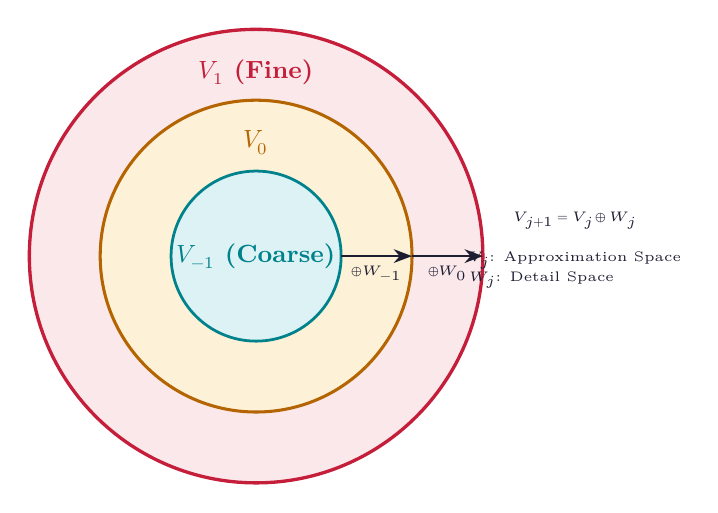
\begin{tikzpicture}[scale=0.9]
  % Nested circles
  \draw[draw=myred, fill=hdrred, line width=1.2pt] (0,0) circle (3.2);
  \draw[draw=myamber, fill=hdramber, line width=1.1pt] (0,0) circle (2.2);
  \draw[draw=myteal, fill=hdrteal, line width=1.0pt] (0,0) circle (1.2);
  
  % Labels
  \node[color=myteal, font=\small\bfseries] at (0, 0) {$V_{-1}$ (Coarse)};
  \node[color=myamber, font=\small\bfseries] at (0, 1.6) {$V_0$};
  \node[color=myred, font=\small\bfseries] at (0, 2.6) {$V_1$ (Fine)};
  
  % Detail space mapping
  \draw[arrow, color=mydark] (1.2, 0) -- (2.2, 0) node[midway, below, font=\tiny] {$\oplus W_{-1}$};
  \draw[arrow, color=mydark] (2.2, 0) -- (3.2, 0) node[midway, below, font=\tiny] {$\oplus W_0$};
  
  \node[font=\tiny\bfseries, color=mydark] at (4.5, 0.5) {$V_{j+1} = V_j \oplus W_j$};
  \node[font=\tiny, color=mydark, align=left] at (4.5, -0.2) {$V_j$: Approximation Space\\$W_j$: Detail Space};
\end{tikzpicture}
\end{tcolorbox}

% ===============================================================================
\section{Scaling Function and Wavelet Function}
% ===============================================================================

An MRA is completely defined by its \textbf{scaling function $\phi(t)$} (also known as the \textbf{Father Wavelet}).

\subsection{The Dilation (Refinement) Equation}
Because $\phi(t) \in V_0 \subset V_1$, and the set $\{\sqrt{2}\phi(2t-k)\}_{k\in\mathbb{Z}}$ forms an orthonormal basis for $V_1$, the scaling function can be expanded as a linear combination of scaled and shifted copies of itself. This is the \textbf{refinement equation} (or \textbf{dilation equation}):
$$\phi(t) = \sqrt{2} \sum_{k=-\infty}^{\infty} h_0[k] \phi(2t - k)$$
where $h_0[k]$ are the \textbf{scaling filter coefficients} (low-pass filter).

\subsection{Detail Spaces ($W_j$) and the Wavelet Function}
The approximation space $V_{j+1}$ has finer resolution than $V_j$. The missing information between them is represented by the \textbf{detail space $W_j$}, defined as the orthogonal complement of $V_j$ in $V_{j+1}$:
$$V_{j+1} = V_j \oplus W_j \quad \text{where } V_j \perp W_j$$
By repeating this decomposition:
$$V_{j+1} = V_{j-1} \oplus W_{j-1} \oplus W_j = V_0 \oplus \bigoplus_{i=0}^{j} W_i$$
To span the detail spaces, we define the \textbf{wavelet function $\psi(t)$} (the \textbf{Mother Wavelet}), which can also be written in terms of the scaling function at the next scale:
$$\psi(t) = \sqrt{2} \sum_{k=-\infty}^{\infty} h_1[k] \phi(2t - k)$$
where $h_1[k]$ are the \textbf{wavelet filter coefficients} (high-pass filter).

% ===============================================================================
\section{The Haar Wavelet System}
% ===============================================================================

The \textbf{Haar system} is the oldest and simplest example of an MRA.

\subsection{Haar Scaling Function (Father Wavelet)}
The Haar scaling function $\phi(t)$ is a simple unit step box function:
$$\phi(t) = \begin{cases} 1 & 0 \le t < 1 \\ 0 & \text{otherwise} \end{cases}$$
Its refinement equation is:
$$\phi(t) = \phi(2t) + \phi(2t-1)$$
Comparing with the general dilation equation $\phi(t) = \sqrt{2}[h_0[0]\phi(2t) + h_0[1]\phi(2t-1)]$, the Haar scaling filter coefficients are:
$$h_0[0] = \frac{1}{\sqrt{2}}, \quad h_0[1] = \frac{1}{\sqrt{2}} \quad (\text{all other } h_0[k] = 0)$$

\subsection{Haar Wavelet Function (Mother Wavelet)}
The Haar wavelet $\psi(t)$ is defined as:
$$\psi(t) = \begin{cases} 1 & 0 \le t < 0.5 \\ -1 & 0.5 \le t < 1 \\ 0 & \text{otherwise} \end{cases}$$
Its refinement equation is:
$$\psi(t) = \phi(2t) - \phi(2t-1)$$
Thus, the Haar wavelet filter coefficients are:
$$h_1[0] = \frac{1}{\sqrt{2}}, \quad h_1[1] = -\frac{1}{\sqrt{2}} \quad (\text{all other } h_1[k] = 0)$$

\begin{tcolorbox}[tikzbox, title={Haar Scaling Function and Wavelet Plots}]
\centering
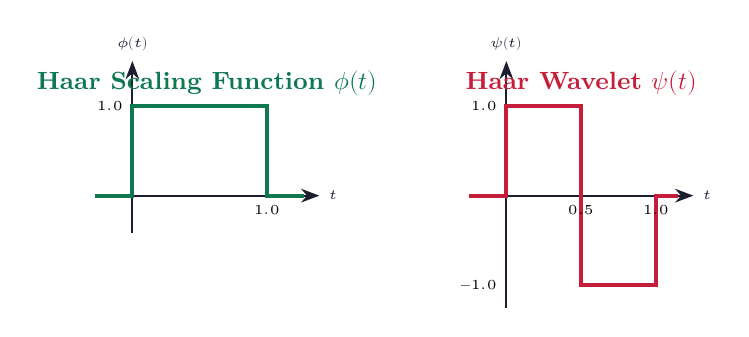
\begin{tikzpicture}[scale=0.95]
  % Scaling Function Plot
  \draw[arrow] (-0.5,0) -- (2.5,0) node[right, font=\tiny] {$t$};
  \draw[arrow] (0,-0.5) -- (0,1.8) node[above, font=\tiny] {$\phi(t)$};
  \draw[line, color=mygreen, line width=1.5pt] (-0.5,0) -- (0,0) -- (0,1.2) -- (1.8,1.2) -- (1.8,0) -- (2.3,0);
  \node[left, font=\tiny] at (0,1.2) {$1.0$};
  \node[below, font=\tiny] at (1.8,0) {$1.0$};
  \node[font=\small\bfseries, color=mygreen] at (1,1.5) {Haar Scaling Function $\phi(t)$};

  % Wavelet Function Plot
  \draw[arrow] (4.5,0) -- (7.5,0) node[right, font=\tiny] {$t$};
  \draw[arrow] (5.0,-1.5) -- (5.0,1.8) node[above, font=\tiny] {$\psi(t)$};
  \draw[line, color=myred, line width=1.5pt] 
    (4.5,0) -- (5.0,0) -- (5.0,1.2) -- (6.0,1.2) -- (6.0,-1.2) -- (7.0,-1.2) -- (7.0,0) -- (7.3,0);
  \node[left, font=\tiny] at (5.0,1.2) {$1.0$};
  \node[left, font=\tiny] at (5.0,-1.2) {$-1.0$};
  \node[below, font=\tiny] at (6.0,0) {$0.5$};
  \node[below, font=\tiny] at (7.0,0) {$1.0$};
  \node[font=\small\bfseries, color=myred] at (6,1.5) {Haar Wavelet $\psi(t)$};
\end{tikzpicture}
\end{tcolorbox}

\subsection{Haar Wavelet Decomposition Example}
Consider a discrete-time signal $x = [c_1, c_2]$ representing values in space $V_1$.
\begin{enumerate}[leftmargin=*, itemsep=4.5pt]
  \item \textbf{Approximation coefficient} (Low-pass projection in $V_0$):
        $$a_1 = \frac{c_1 + c_2}{\sqrt{2}}$$
  \item \textbf{Detail coefficient} (High-pass projection in $W_0$):
        $$d_1 = \frac{c_1 - c_2}{\sqrt{2}}$$
\end{enumerate}
The Haar transform maps $[c_1, c_2] \to [a_1, d_1]$. It decomposes the signal into its local mean (coarse trend) and local difference (detail fluctuation).

\subsection{Haar Wavelet Packets and Applications}
A standard Haar DWT only decomposes the low-pass approximation coefficients ($a_j$) recursively. A \textbf{Haar Wavelet Packet} decomposition recursively filters both the approximation ($a_j$) and the detail ($d_j$) coefficients at each level, yielding a full balanced binary tree.

\subsubsection{Recursive Generation of Haar Wavelet Packets}
Let $W_0(t) = \phi(t)$ be the Haar scaling function and $W_1(t) = \psi(t)$ be the Haar wavelet function. The higher-order wavelet packet functions $W_n(t)$ for $n \ge 0$ are recursively defined by:
$$W_{2n}(t) = \sum_{k=0}^{1} h_0[k] W_n(2t - k) = \frac{1}{\sqrt{2}} \left[ W_n(2t) + W_n(2t-1) \right]$$
$$W_{2n+1}(t) = \sum_{k=0}^{1} h_1[k] W_n(2t - k) = \frac{1}{\sqrt{2}} \left[ W_n(2t) - W_n(2t-1) \right]$$
For example, starting from the first level:
\begin{itemize}[leftmargin=*, itemsep=2pt]
  \item $W_2(t)$ is generated from the low-pass projection of $W_1(t)$, representing a high-frequency approximation packet.
  \item $W_3(t)$ is generated from the high-pass projection of $W_1(t)$, representing a high-frequency detail packet.
\end{itemize}

\subsubsection{Applications of Haar Wavelet Packets}
Due to their simple step-like structure and ease of computational implementation, Haar wavelet packets are widely used in:
\begin{itemize}[leftmargin=*, itemsep=3.5pt]
  \item \textbf{Transient Signal Detection:} The localized rectangular support of Haar packets makes them highly sensitive to sudden spikes, edges, and discontinuities in signals.
  \item \textbf{High-Frequency Feature Extraction:} By decomposing the high-frequency bands recursively, Haar packets capture structural texture details in images that standard DWT skips.
  \item \textbf{Real-Time Low-Power Hardware Implementations:} Since the Haar filter coefficients ($1/\sqrt{2}$) involve simple additions and subtractions, Haar packet transforms are ideal for low-cost hardware implementation on microcontrollers and FPGAs.
\end{itemize}

\newpage
% ===============================================================================
\begin{center}
  {\large\bfseries\color{myred} Quick Revision --- Module 3}\\[3pt]
  {\small\color{mydark} Discrete Wavelet Transform \& MRA $|$ PE-EC703C}
\end{center}
\noindent{\color{myred}\rule{\linewidth}{1.2pt}}
\vspace{4pt}
% ===============================================================================

\begin{tcolorbox}[formulabox, title={\textbf{Key DWT \& MRA Equations}}]
\renewcommand{\arraystretch}{1.35}
\begin{tabularx}{\linewidth}{B{5.0cm} X}
MRA Nested Spaces & $\dots \subset V_{-1} \subset V_0 \subset V_1 \subset V_2 \dots \subset L^2(\mathbb{R})$ \\[4pt]
Scaling Refinement Eq. & $\phi(t) = \sqrt{2} \sum_{k} h_0[k] \phi(2t - k) \quad$ (Father Wavelet) \\[4pt]
Wavelet Refinement Eq. & $\psi(t) = \sqrt{2} \sum_{k} h_1[k] \phi(2t - k) \quad$ (Mother Wavelet) \\[4pt]
Orthogonal Complement & $V_{j+1} = V_j \oplus W_j \quad$ where $V_j \perp W_j$ \\[4pt]
Haar scaling coefficients & $h_0[0] = 1/\sqrt{2}, \quad h_0[1] = 1/\sqrt{2}$ \\[4pt]
Haar wavelet coefficients & $h_1[0] = 1/\sqrt{2}, \quad h_1[1] = -1/\sqrt{2}$
\end{tabularx}
\tcbset{after={\color{black}}}
\end{tcolorbox}

\begin{tcolorbox}[defbox, title={\textbf{One-Line Definitions}}]
\begin{itemize}[leftmargin=*, itemsep=3.5pt]
  \item \textbf{MRA:} A mathematical framework decomposing a signal into nested resolution spaces.
  \item \textbf{Approximation Space ($V_j$):} Subspace containing low-resolution signal trends up to scale $j$.
  \item \textbf{Detail Space ($W_j$):} Subspace containing the localized high-resolution differences between $V_j$ and $V_{j+1}$.
  \item \textbf{Father Wavelet ($\phi(t)$):} The scaling function that spans the approximation spaces.
  \item \textbf{Mother Wavelet ($\psi(t)$):} The wavelet function that spans the detail spaces.
  \item \textbf{Dilation Equation:} A recursive relation defining the scaling function using scaled/shifted copies of itself.
  \item \textbf{Haar Wavelet:} The simplest orthonormal wavelet, represented by an asymmetric step function.
\end{itemize}
\end{tcolorbox}

\begin{tcolorbox}[exambox, title={\textbf{Frequently Asked / Viva Questions}}]
\begin{enumerate}[topsep=0pt, label=\textbf{Q\arabic*.}, itemsep=5pt]
  \item \Q{State the five basic axioms of Multi-resolution Analysis (MRA).}
        The five axioms are: (1) Containment: $V_j \subset V_{j+1}$; (2) Completeness: $\bigcap V_j = \{0\}$; (3) Density: $\overline{\bigcup V_j} = L^2(\mathbb{R})$; (4) Scaling Similarity: $f(t) \in V_j \iff f(2t) \in V_{j+1}$; and (5) Translation Invariance: $f(t) \in V_0 \iff f(t-k) \in V_0$.

  \item \Q{What is the difference between approximation space and detail space?}
        The approximation space ($V_j$) represents the low-frequency, smoothed version of a signal at resolution scale $j$. The detail space ($W_j$) represents the high-frequency difference or fluctuation needed to transition from a coarse scale $V_j$ to a finer scale $V_{j+1}$.

  \item \Q{Write down the refinement/dilation equation for the scaling function.}
        The refinement equation is: $\phi(t) = \sqrt{2} \sum_{k=-\infty}^{\infty} h_0[k] \phi(2t-k)$, where $h_0[k]$ are the scaling filter coefficients. This equation shows that the scaling function is self-similar across scales.

  \item \Q{What are the coefficients of the Haar scaling and wavelet filters?}
        For the Haar scaling filter: $h_0[0] = 1/\sqrt{2}$, $h_0[1] = 1/\sqrt{2}$. For the Haar wavelet filter: $h_1[0] = 1/\sqrt{2}$, $h_1[1] = -1/\sqrt{2}$. All other coefficients are zero.

  \item \Q{Why does the DWT avoid the redundancy of the CWT?}
        The CWT varies the scale $a$ and shift $b$ continuously, creating infinite overlap and redundant representation. The DWT samples the time-scale grid discretely (usually on a dyadic grid: $a = 2^j, b = k \cdot 2^j$), creating an orthogonal, non-redundant representation.

  \item \Q{What is the relation between the scaling function $\phi(t)$ and the wavelet function $\psi(t)$?}
        The scaling function $\phi(t)$ generates the approximation spaces ($V_j$). The wavelet function $\psi(t)$ is orthogonal to $\phi(t)$ and generates the detail spaces ($W_j$). Mathematically, $\psi(t)$ is derived from the scaling function via: $\psi(t) = \sqrt{2} \sum_{k} h_1[k] \phi(2t-k)$.

  \item \Q{What are the drawbacks of the Haar wavelet system?}
        The Haar wavelet is discontinuous in the time domain, which causes poor frequency resolution and spectral leakage. Additionally, it has only one vanishing moment, making it inefficient for compressing smooth signals.
\end{enumerate}
\end{tcolorbox}

\begin{tcolorbox}[tikzbox, title={\textbf{Comparison Table: Approximation vs. Detail Spaces}}]
\par\noindent
{\renewcommand{\arraystretch}{1.4}%
\begin{tabularx}{\linewidth}{|B{3.2cm}|Y|Y|}
\hline
\textbf{Feature} & \textbf{Approximation Space ($V_j$)} & \textbf{Detail Space ($W_j$)} \\
\hline
\textbf{Spanning Basis} & Shifted Scaling Functions: $\{\phi_{j,k}(t)\}$. & Shifted Wavelet Functions: $\{\psi_{j,k}(t)\}$. \\
\hline
\textbf{Spectral Content} & Low-frequency components (trends). & High-frequency components (details/edges). \\
\hline
\textbf{Filtering Operation} & Low-pass filter ($h_0[k]$). & High-pass filter ($h_1[k]$). \\
\hline
\textbf{Relationship} & $V_{j+1} = V_j \oplus W_j$ & $W_j \perp V_j$ and $W_j \perp W_i$ (for $i \neq j$). \\
\hline
\end{tabularx}}
\end{tcolorbox}

\end{document}
